%! Author = Frederik Bußmann
%! Date = 22.06.2023

\section{Anhang I: Übersicht der verwendeten CI-Tools} \label{sec:appendix-1}

In Kapitel\ \ref{subsec:04-implementation-2} wurden verschiedene\ \acrshort{ci}-Tools und Services vorgestellt, welche
für die Fallstudie zur Umsetzung der Strategie eingesetzt wurden.
Im Folgenden wird eine Übersicht der genutzten Tools und dessen Funktionen und Merkmale gegeben:

\subsection*{Version-Control-System und Pipeline-Runner}

\begin{itemize}
    \item {
        \textbf{GitLab}\par
        GitLab ist ein webbasierter Service für Versionierung mit dem\ \acrshort{vcs}\ \glqq Git\grqq.
        Es bietet alle verteilten Versionskontroll- und Quellcodeverwaltungsfunktionen von Git sowie einige zusätzliche
        Features.
        Dies umfasst zum Beispiel eine Zugriffskontrolle und mehrere Kollaborationsfunktionen wie Aufgabenverwaltung,
        Fehlerverfolgung und Feature-Anfragen für Projekte sowie eine integrierte Wiki-Funktion für die
        Dokumentation.
        Der Service bietet außerdem \acrshort{ci}-Tools und Pipeline-Verwaltung an.
        Dieser wird unter einer Open-Source-Lizenz vertrieben und dessen Self-Managed-Version ermöglicht es,
        GitLab auf eigenen Servern zu installieren und zu verwalten.\footpartcite{gitlab}
    }

    \item {
        \textbf{GitLab CI/CD}\par
        GitLab CI/CD ist der Pipeline-Runner von GitLab und stellt eine eingebaute Pipeline-Lösung für das Ausführen von
        \acrshort{ci}- und \acrshort{cd}-Prozessen dar.
        Das Tool ist vollständig in GitLab integriert und verwendet eine Konfigurationsdatei innerhalb des
        Repositories, um die Phasen und Jobs der \acrshort{ci}-Pipelines zu definieren.
        Es bietet eine breite Palette von Funktionen, einschließlich der Parallelisierung von Jobs, Pipelines für
        unterschiedliche Branches und das Verwalten von Umgebungsvariablen.
        GitLab CI/CD kann auf eigenen Servern oder in der Cloud ausgeführt werden, und sowohl für bei GitLab, als auch
        für extern gehostete Repositorys verwendet werden, was es zu einer flexiblen Lösung macht.
        Die für das Ausführen der Pipeline benötigten Umgebungsvariablen, Passwörter und andere vertrauliche Daten
        können dabei in einer von GitLab zur Verfügung gestellten, sicheren Datenbank verwaltet werden.
        \footpartcite{gitlab-ci-cd}
    }
\end{itemize}

\subsection*{Software-Testing}

\begin{itemize}
    \item {
        \textbf{PHPUnit}\par
        PHPUnit ist ein weitverbreitetes Open-Source Unit-Testing-Framework, welches zum Erstellen von
        Unit-Tests in PHP-basierten Applikationen verwendet wird.
        Das Framework ermöglicht das Erstellen von Mocks und das Auswerten der Test-Coverage für das zu
        testende Projekt.
        \footpartcite{phpunit}
    }

    \item {
        \textbf{Infection}\par
        Infection ist eine Mutation-Testing-Library für PHP.
        Sie ändert den Quellcode automatisch und führt dann bestehende Tests erneut aus, um zu sehen, ob diese
        fehlschlagen.
        Wenn die Tests bestehen, obwohl der Code mutiert wurde, zeigt Infection diese Stellen im Code an, damit
        diese verbessert werden können.
        Die Library unterstützt die Integration mit PHPUnit und weiteren Testing-Tools.
        \footpartcite{infection}
    }

    \item {
        \textbf{Jest}\par
        Jest ist ein Javascript Testing-Framework und ermöglicht das Einbringen von Unit-Tests in
        JavaScript-basierten Applikationen.
        Ähnlich wie PHPUnit unterstützt Jest das Erstellen von Mocks und bietet Funktionen zur Coverage an.
        Das Framework parallelisiert laufende Tests, um eine möglichst hohe Performance zu bieten.
        \footpartcite{jest}
    }

    \item {
        \textbf{Cypress}\par
        Cypress ist ein Framework für Webapplikationen, um Functional-Tests durchzuführen.
        Es ermöglicht das automatisierte Testen von Benutzerinteraktionen innerhalb einer Webapplikation in
        einem realen Browser.
        Durch Cypress kann das Zusammenspiels des gesamten Projekts prüfen und zur Automatisierung
        von Testfällen genutzt werden, bei denen normalerweise Nutzer-Interaktion erforderlich ist.
        \footpartcite{cypress}
        Shopware bietet eine eigene Test-Suite für System-Tests durch Cypress an.\footpartcite{shopware-cypress}
    }
\end{itemize}

\subsection*{Static-Code-Analysis}

\begin{itemize}
    \item {
        \textbf{PHP\_CodeSniffer}\par
        \acrfull{phpcs} ist ein Set aus zwei Kommandozeilen-Befehlen für das Analysieren von PHP-
        und JavaScript-Code und von \acrfull{css} nach einem gegebenen Coding-Standard und für
        das automatische Korrigieren von Abweichungen dieses Standards.
        Das Tool kann mit vorgegebenen und eigens erstellten oder angepassten Regelsätzen betrieben werden.
        \footpartcite{php-codesniffer}
    }

    \item {
        \textbf{PHP Mess Detector}\par
        \acrfull{phpmd} ist eine Software, die nach vorgegebenen Problemen und Unstimmigkeiten in
        PHP-Code sucht.
        Das Tool kann zum Verhindern des Einführens von überflüssigen Variablen und Methoden, unoptimiertem Code und
        möglichen Fehlern in die Zielumgebung genutzt werden.
        \acrshort{phpmd} kann ergänzend zu Danger und \acrshort{phpcs} zur statischen Analyse von PHP-Code verwendet
        werden.\footpartcite{php-mess-detector}
    }

    \item {
        \textbf{PHPStan}\par
        PHPStan ist ein weiteres \acrshort{qa}-Tool für das statische Analysieren von PHP-Code.
        Es konzentriert sich auf die Erkennung von Fehlern, die im laufenden Betrieb zu Problemen führen können, wie
        z. B. Aufrufe von nicht existierenden Methoden, ungenutzte Variablen etc.
        PHPStan kann in den Entwicklungsprozess integriert werden, um die Codequalität kontinuierlich zu verbessern.
        \footpartcite{phpstan}
    }

    \item {
        \textbf{Deptrac}\par
        Deptrac ist ein statisches Code-Analyse-Tool, das dabei hilft, die Architektur eines PHP-Projekts zu verstehen
        und zu überprüfen.
        Es stellt sicher, dass die Abhängigkeiten zwischen den Modulen eines Projekts den definierten Architekturregeln
        entsprechen.
        Deptrac kann in den Entwicklungsprozess integriert werden, um die Architektur des Projekts kontinuierlich zu
        überwachen und zu verbessern.\footpartcite{deptrac}
    }

    \item {
        \textbf{Eslint}\par
        ESLint ist ein statisches Tool zur Analyse von JavaScript-Code.
        Das Tool ist sehr anpassbar und kann für das Entwickeln mit verschiedenen Frameworks und Libraries genutzt
        werden.
        Viele Text- und Code-Editoren unterstützen ESLint und zeigen Analyse-Resultate bereits bei der Entwicklung im Editor
        an.
        Das Tool unterstützt außerdem das automatische Beheben von bestimmten Syntax-Fehlern mit einem eingebauten
        Kommandozeilenbefehl.\footpartcite{eslint}
    }

    \item {
        \textbf{Danger JS}\par
        Danger ist ein statisches Analyse-Tool, welches direkt in \acrshort{vcs} angebunden werden kann.
        Das Tool läuft während des \acrshort{ci}-Prozesses und kann zur Automatisierung von Code-Review-Aufgaben
        genutzt werden.
        Mit Danger können Warnungen und Fehler in der Pipeline geworfen werden, wenn geplante Integrationen zu
        groß werden, kein Changelog-Eintrag für Änderungen angelegt wurde, Abhängigkeiten nicht up to date sind und
        vieles mehr.
        Danger kann außerdem Job-Ergebnisse einer Pipeline in Form von Kommentaren in Merge-Requests hinterlegen,
        um Entwickler schneller über den Status des Projekts zu informieren.
        Die Software wird für die Programmiersprachen JavaScript, Ruby, Kotlin, Python und Swift angeboten.
        \footpartcite{danger-js}
    }

    \item {
        \textbf{License Checker}\par
        License Checker sind Tools, die Lizenzen von Abhängigkeiten in einem Projekt überprüfen.
        Sie können dabei helfen, Lizenzprobleme bei Plugins und Erweiterungen von Drittanbietern zu identifizieren
        und zu vermeiden.
        Für das Prüfen von Composer- und\ \acrshort{npm}-Paketen existieren jeweils eigene PHP- und JavaScript-basierte
        Tools.
        \footpartcite{php-license-checker}\textsuperscript{,\ }\footpartcite{js-license-checker}
    }

    \item {
        \textbf{Security Checker / AuditJS}\par
        Security Checker sind Tools, die überprüfen, ob die in einem Projekt verwendeten Abhängigkeiten bekannte
        Sicherheitslücken aufweisen.
        Diese Tools können dabei helfen, Projekte kontinuierlich zu überwachen und sicher zu halten.
        Symfony bietet für das automatische Prüfen von Applikationen einen eigenen Security Checker.
        \footpartcite{symfony-security-checker}
        Darüber hinaus wurde zur Prüfung von JavaScript-Abhängigkeiten in der Fallstudie das JavaScript-basierte
        Sicherheitsprüfungs-Tool AuditJS verwendet.
        \footpartcite{audit-js}
    }
\end{itemize}

\clearpage

\subsection*{Deployment}

\begin{itemize}
    \item {
        \textbf{Deployer}\par
        Deployer ist ein PHP-basiertes Deployment-Tool, welches zur automatisierten Auslieferung von Software an
        verschiedene Umgebungen verwendet werden kann.
        Das Werkzeug bietet vordefinierte Setups für das Deployment verschiedener Services und weitere wichtige
        Features wie minimale Ausfallzeiten und die Möglichkeit, ausgelieferte Software auf einen früheren Stand
        zurückzurollen.
        \footpartcite{deployer}
        Shopware stellt eine Anleitung für das Einsetzen von Deployer in Projekten bereit, wobei auch die Nutzung mit
        GitLab CI/CD abgedeckt wird.
        \footpartcite{shopware-deployer}
    }
\end{itemize}

\clearpage

\section{Anhang II: Darstellung ausgeführter Pipelines} \label{sec:appendix-2}

Der für die Umsetzung der Fallstudie gewählte Pipeline-Runner GitLab CI/CD bietet eine Übersicht aller
Pipeline-Instanzen, die im Verlauf des Projekts durchgeführt wurden.
Neben dem Titel und der Art des Ausgangs-Branches der Pipeline wird hierbei auch der Status der Pipeline aufgezeigt:

\begin{figure}[H]
    \centering
    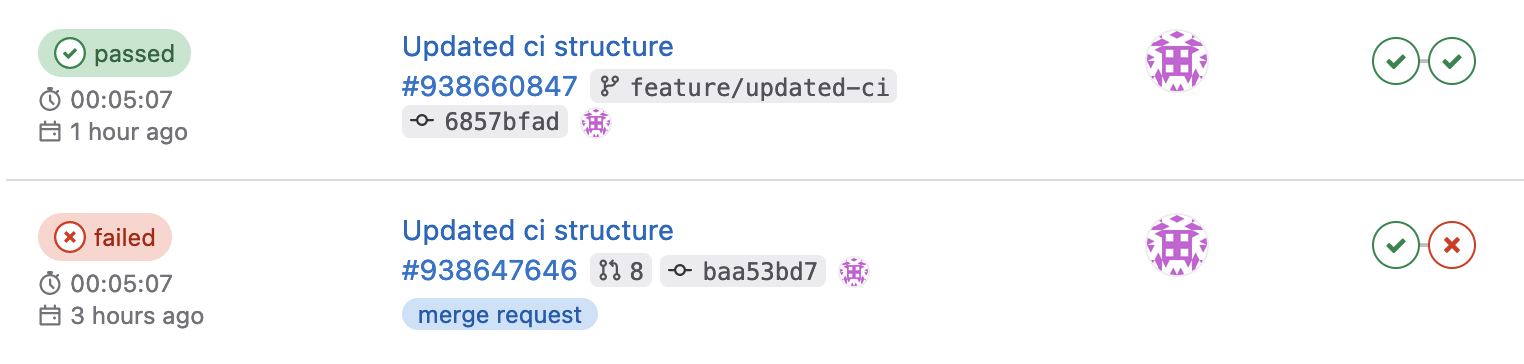
\includegraphics[width=\textwidth]{images/content/pipeline-overview}
    \captioncite[\hyperlink{cite.gitlab}{GitLab B.V.}]{}{Übersicht ausgeführter Pipelines in GitLab CI/CD}
    \label{fig:pipeline-overview}
\end{figure}

Abbildung\ \ref{fig:pipeline-overview} stellt einen Ausschnitt der Pipeline-Übersicht dar.
Es werden zwei verschiedene Pipelines angezeigt, wobei eine erfolgreich durchgeführt und die andere
aufgrund von Fehlern in einem der Jobs abgebrochen wurde.
Die fehlgeschlagene Pipeline wird dabei durch ein rotes X mit dem Schriftzug\ \glqq failed\grqq\ markiert, während die
erfolgreich durchgelaufene Pipeline einen grünen Haken und das Wort\ \glqq passed\grqq\ ausgibt.
\\\\
Navigiert man in der Pipeline-Auflistung von GitLab CI/CD zu der Detail-Ansicht einer der gezeigten Pipelines, werden
dessen Phasen und Jobs dargestellt.
Die hierbei angezeigten Jobs können entweder als erfolgreich oder fehlerhaft markiert werden:

\begin{figure}[H]
    \centering
    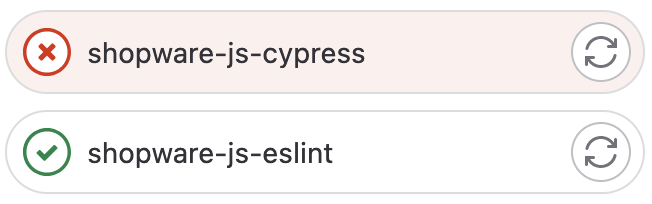
\includegraphics[width=0.5\textwidth]{images/content/job-status}
    \captioncite[\hyperlink{cite.gitlab}{GitLab B.V.}]{}{Status-Anzeige der Jobs einer Pipeline}
    \label{fig:job-status}
\end{figure}

In Abbildung\ \ref{fig:job-status} werden verschiedene Jobs aufgezeigt, welche jeweils einen unterschiedlichen Status
berichten.
Während der Job für das statische Code-Analyse-Tool Eslint erfolgreich durchgelaufen ist, wurde der Job zur
Durchführung von System-Tests durch Cypress abgebrochen.
Der erfolgreiche Job wird hierbei mit einem grünen Haken markiert, während der abgebrochene Job mit einem roten X
gekennzeichnet wurde.
\\\\
Neben den Job-Informationen werden in der Pipeline-Detail-Ansicht noch weitere Metriken wie die Anzahl der in den Jobs
durchgeführten Tests oder die Dauer der gesamten Pipeline ausgegeben.
Eine Übersicht aller Jobs einer ausgewählten Pipeline wird in Abbildung\ \ref{fig:job-overview} angezeigt.
Diese implementiert die in Kapitel\ \ref{subsec:04-implementation-2} ausgewählten Tools der \acrshort{ci}-Strategie,
welche nach dem erfolgreichen Build-Job in der Testing-Phase der Pipeline stattfinden.
Jobs können in dieser Detail-Ansicht wiederholt und manche manuell angestoßen werden, wie zum Beispiel der
Deployment-Job für die Development-Umgebung, welcher in der Deployment-Phase der Pipeline ausführbar ist.
Dieser kann von den Entwicklern auf der Web-Oberfläche gestartet werden, um die gebaute und getestete Integration an die
hinterlegte Umgebung auszuliefern.

\begin{figure}[H]
    \centering
    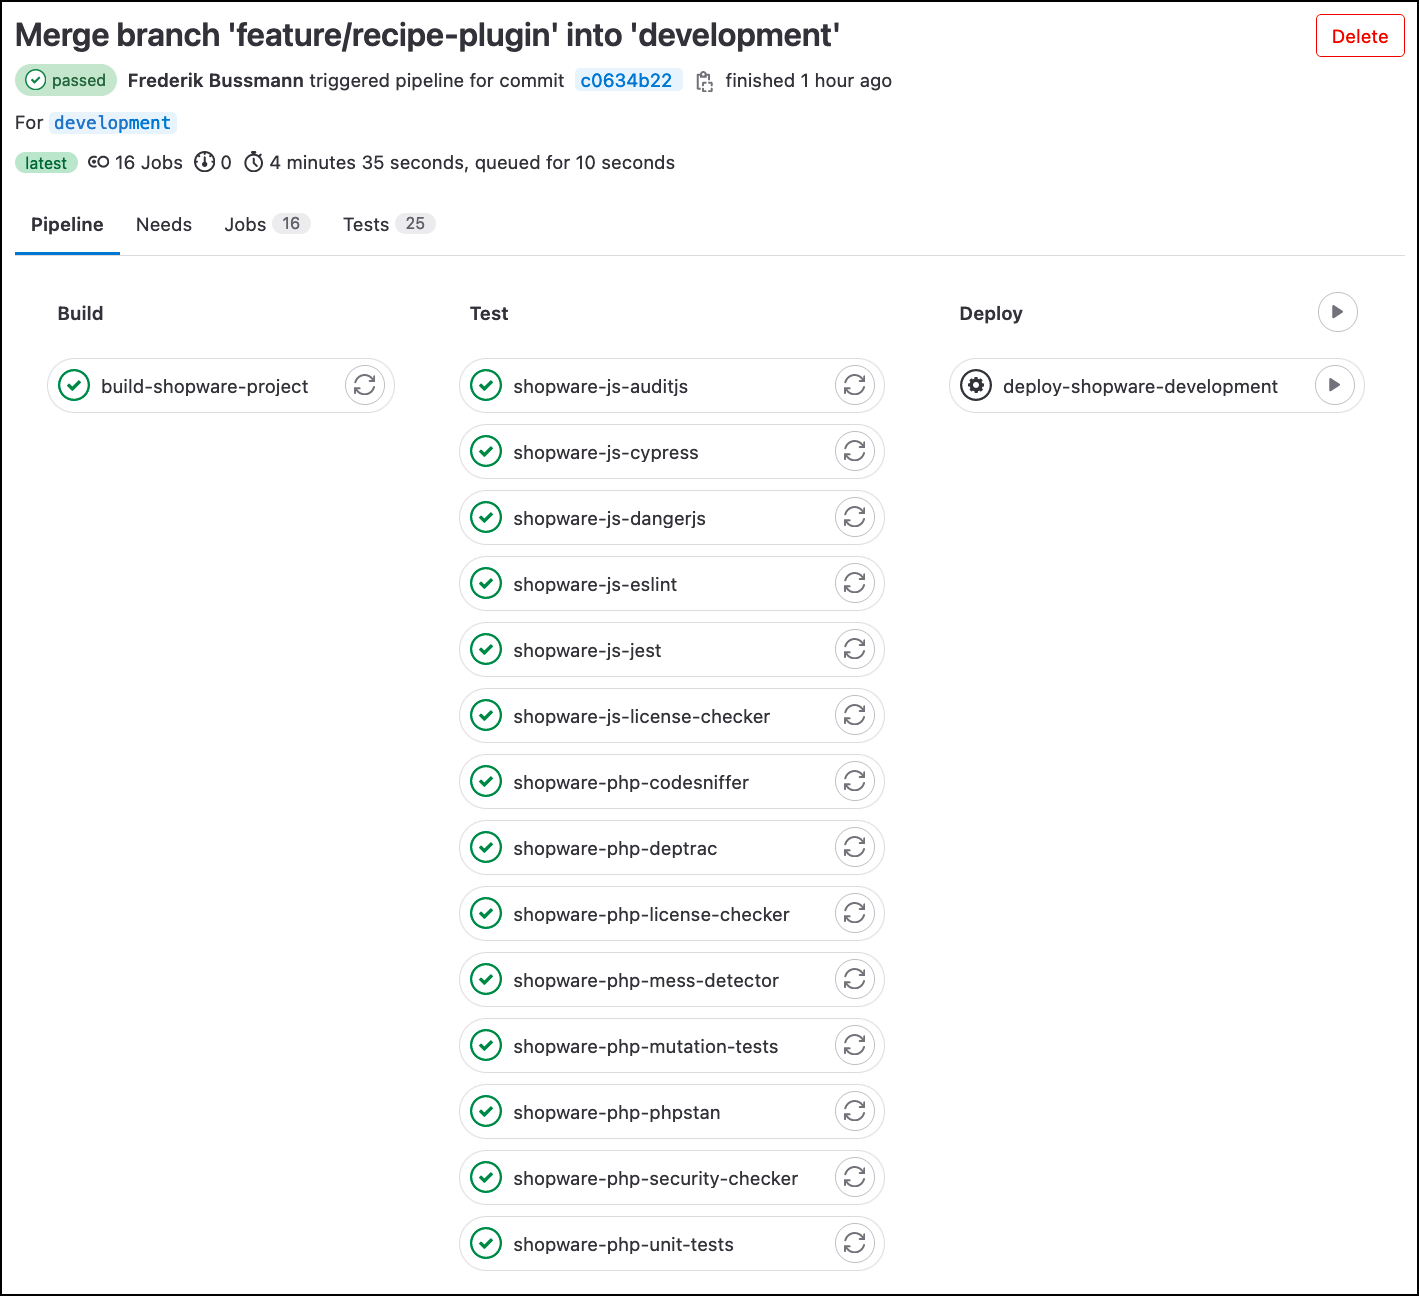
\includegraphics[width=\textwidth]{images/content/job-overview}
    \captioncite[\hyperlink{cite.gitlab}{GitLab B.V.}]{}{Detail-Ansicht einer durchgeführten Pipeline}
    \label{fig:job-overview}
\end{figure}
